\begin{frame}
  \frametitle{Table of Contents}
  \begin{itemize}
  \item <1-> Add some contents....
  \end{itemize}
\end{frame}

\begin{frame}
  \frametitle{More online}
  \begin{center}
    \begin{figure}[t]
      \centering
      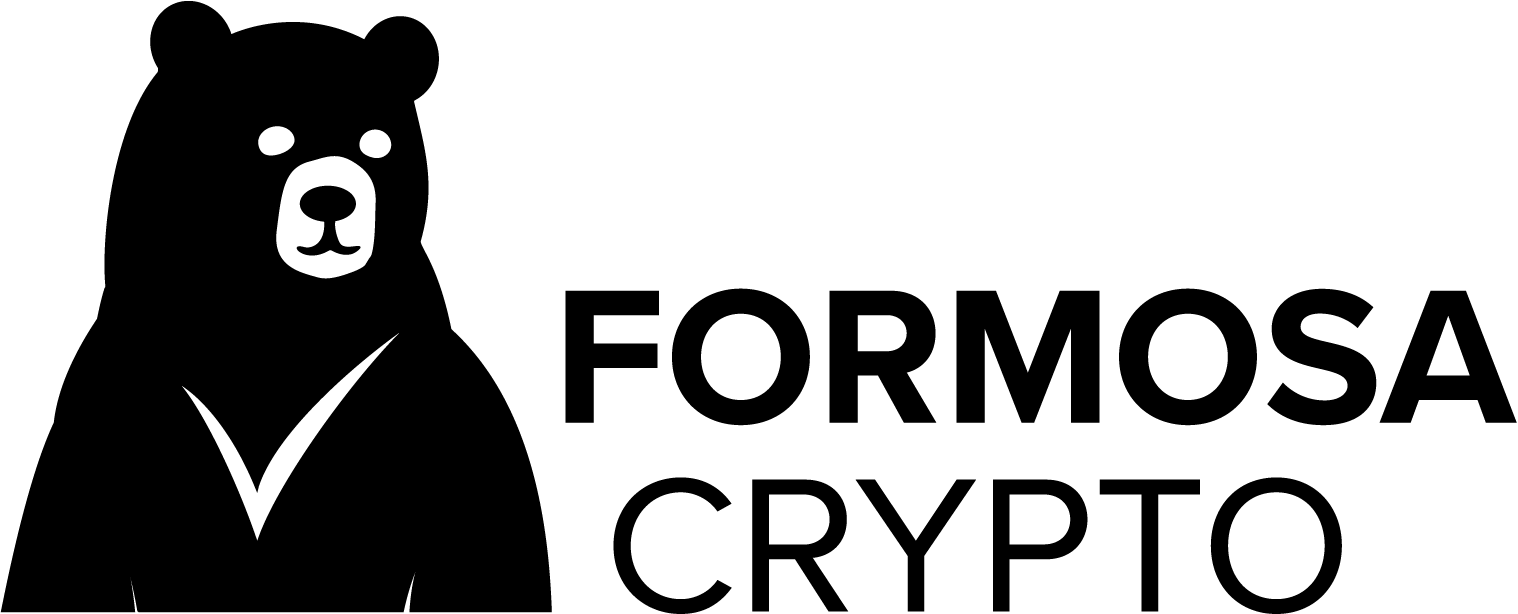
\includegraphics[width=0.5\textwidth]{formosa}
      \caption*{\Large \url{https://formosa-crypto.org}}
    \end{figure}
  \end{center}
  \vspace*{.5cm}
  \begin{itemize}
  \item \textbf{EasyCrypt specifications}: \url{https://github.com/formosa-crypto/crypto-specs}
  \item \textbf{Libjade:} \url{https://github.com/formosa-crypto/libjade}
  \end{itemize}
\end{frame}

% \frame[plain,allowframebreaks]{
% % \frametitle{References}
% % citations from table
% \bibliography{bib/abbrev0.bib,bib/crypto.bib}
% }

